%%%%%%%%%%%%%%%%%%%%%%%%%%%%%%%%%%%%%%%%%%%%%%%%%%%%%%
  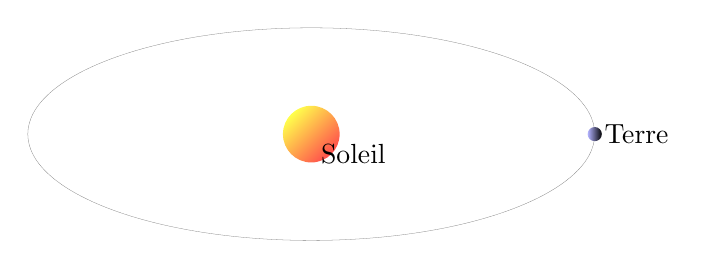
\begin{tikzpicture}[scale=0.9]

    \coordinate (e1) at (3,3);
    \coordinate (e2) at (7,3);
    \def\rayonS{0.4}
    \def\rayonT{0.1}
  % Soleil
  \shade[
    top color=yellow!70,
    bottom color=red!70,
    shading angle={45},
   ] (e1) circle (\rayonS);
   \draw (e1) node[below right] {Soleil};

  % Draw the elliptical path of the Earth.
  \draw[ultra thin, gray] (e1) ellipse (4 and 1.5);
  	
  % Terre
  \shade[
          top color=black,
          bottom color=blue!30,
          shading angle={-90},
        ] (e2) circle (\rayonT);
  \draw (e2) node[right] {Terre};
  \end{tikzpicture}
%%%%%%%%%%%%%%%%%%%%%%%%%%%%%%%%%%%%%%%%%%%%%%%%%%%%%%%%%%%%%%%%%%%%
